\documentclass[border=4pt]{standalone}
\usepackage{amsmath,amssymb,amsfonts}
\usepackage{xcolor,colortbl,array,booktabs,multirow}
\usepackage{tikz}
\usepackage{pgfplots}
\pgfplotsset{compat=1.16}
\usetikzlibrary{arrows, automata, backgrounds, calendar, chains, decorations,
    matrix, mindmap, patterns, petri, positioning, shadows, shapes.geometric,
    trees, shapes, decorations.pathreplacing, calc, tikzmark, arrows.meta,
    intersections, fit, graphs, quotes, angles, decorations.markings}
\newcommand{\st}{\text{ s.t. }}
\newcommand{\x}{\mathbf{x}}
\renewcommand{\b}{\mathbf{b}}
\renewcommand{\c}{\mathbf{c}}
\newcommand{\A}{\mathbf{A}}
\newcommand{\y}{\mathbf{y}}
\newcommand{\z}{\mathbf{z}}
\newcommand{\R}{\mathbb{R}}
\newcommand{\RR}{\mathbb{R}}
\newcommand{\Z}{\mathbb{Z}}
\newcommand{\ZZ}{\mathbb{Z}}
\newcommand{\npcomplete}{NP-complete}
\providecommand{\true}{\text{TRUE}}
\providecommand{\false}{\text{FALSE}}
\tikzset{vertex/.style={circle,fill=black!25,minimum size=20pt,inner sep=0pt},
    edge/.style={draw,thick,-},weight/.style={font=\small},
    selected vertex/.style={vertex, fill=red!24},
    selected edge/.style={draw,line width=2pt,-,red!50},
    ignored edge/.style={draw,line width=2pt,-,black!20}}
\newcommand{\vect}{\vec}
\providecommand{\ds}{\displaystyle}
\providecommand{\longvect}{\overrightarrow}
\usepackage[normalem]{ulem}
\definecolor{ocre}{RGB}{243,102,25}
\providecommand{\leftB}{\left[}
\providecommand{\rightB}{\right]}
\tikzset{directed/.style={postaction={decorate,decoration={markings,mark=at position .65 with {\arrow{>}}}}},
    directed1/.style={postaction={decorate,decoration={markings,mark=at position .65 with {\arrow{>}}}}}}
\begin{document}
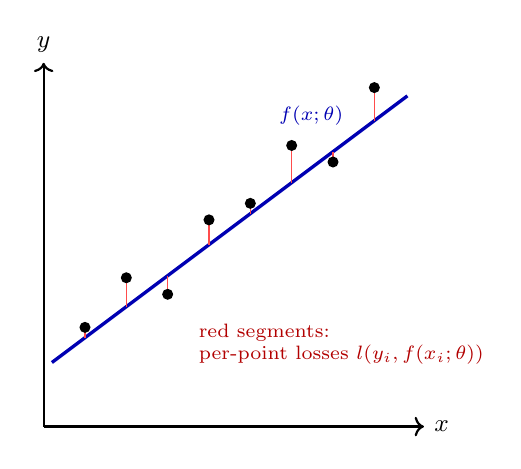
\begin{tikzpicture}[scale=1.05]
  % axes
  \draw[->, thick] (0,0) -- (4.6,0) node[right] {\small $x$};
  \draw[->, thick] (0,0) -- (0,4.4) node[above] {\small $y$};
  % fitted line y = 0.75x + 0.7
  \draw[blue!70!black, very thick] (0.1,0.775) -- (4.4,4.0) node[pos=0.85, above left, font=\scriptsize, text=blue!70!black] {$f(x;\theta)$};
  % data points and residuals
  \foreach \x/\y in {0.5/1.2, 1.0/1.8, 1.5/1.6, 2.0/2.5, 2.5/2.7, 3.0/3.4, 3.5/3.2, 4.0/4.1}{
    \pgfmathsetmacro\fy{0.75*\x + 0.7}
    \draw[red!70, thin] (\x,\y) -- (\x,\fy);
    \fill[black] (\x,\y) circle (1.9pt);
  }
  \node[font=\scriptsize, text=red!70!black, align=left] at (3.6,1.0) {red segments:\\ per-point losses $l(y_i, f(x_i;\theta))$};
\end{tikzpicture}
\end{document}
